\documentclass{article}


% if you need to pass options to natbib, use, e.g.:
%     \PassOptionsToPackage{numbers, compress}{natbib}
% before loading DSA_2024


% ready for submission
\usepackage[final]{DSA_2024}

\usepackage[utf8]{inputenc} % allow utf-8 input
\usepackage[T1]{fontenc}    % use 8-bit T1 fonts
\usepackage{hyperref}       % hyperlinks
\usepackage{url}            % simple URL typesetting
\usepackage{booktabs}       % professional-quality tables
\usepackage{amsfonts}       % blackboard math symbols
\usepackage{nicefrac}       % compact symbols for 1/2, etc.
\usepackage{microtype}      % microtypography
\usepackage{xcolor}         % colors
\usepackage[pdftex]{graphicx}
\usepackage{fancyvrb}
\title{Unlocking Biomedical Data for AI Health Research in Africa Using GeneNetwork as an Example}

\author{%
  Munyoki Kilyungi\thanks{\url{https://bonfacemunyoki.com}} \\
  Strathmore University\\
  Nairobi, Kenya \\
  \texttt{me@bonfacemunyoki.com} \\
  \And
  Pjotr Prins\thanks{\url{https://thebird.nl}} \\
  The University of Tennessee Health Science Center \\
  Memphis, TN \\
  \texttt{jprins@uthsc.edu} \\
  \AND
  Solomon Shelby \\
  The University of Tennessee Health Science Center \\
  Memphis, TN \\
  \texttt{ssd2024@nyeusi.tech} \\
}

\begin{document}
\maketitle

\begin{abstract}

  The GeneNetwork (GN) database contains over two decades of experimental data from genetics, phenotyping, Quantitative Trait Locus (QTL) and Genome Wide Association (GWA) studies in human and model species, such as mouse and rat.  However, this data is currently difficult to access and manipulate due to its complex underlying structures, including around 80 cross-referenced SQL tables and various file types.  In our work, we show how we re-organise this data into a graph-based model, thereby providing automated data discovery that align with the principles of Findability, Accessibility, Interoperability, and Reusability (FAIR).  This novel approach allows for the creation of a more flexible GN service which can automatically infer relationships between disparate data elements.  This feature can serve as the input for Large Language Models due to its adherence to FAIR principles.

\textbf{\textsc{Keywords:}} \textit{Artificial Intelligence, Data Accessibility, Data Interpretation, GeneNetwork, Biological Data, Data Discovery, Resource Description Framework (RDF), Metadata}
\end{abstract}


\section{Introduction}

Genetic data analysis is important for understanding the underlying mechanisms of various biological processes and diseases.  Genenetwork2 (\url{https://genenetwork.org}) is a powerful open-source software platform that provides a range of tools and resources for analysing, visualising and storing genetic data, mostly written in the python programming language with a SQL database and flat files as a backend \cite{mulligan2017genenetwork}\cite{sloan2016genenetwork}.  It contains over 20 years of experimental data from genetics, phenotyping, QTL and GWA studies in human and model species such as mouse and rat \cite{sloan2016genenetwork}.  The size of the data is about 1TB and growing about 20\% a year.  The current SQL database underlying GN can be complex and difficult to write software against, and lacks interoperability with other systems.

The Resource Description Framework (RDF) is a widely-used graph based semantic data model that can provide several benefits over SQL, including support for complex data types, reasoning and ontologies \cite{allemang2011semantic}\cite{candan2001resource}.  Representing GN's data in RDF has the potential to enable more flexible querying, data integration and reasoning capabilities, as well as better support for Linked Data and Semantic Web standards.  RDF is particularly suitable for machine learning and AI because it allows machines/software to analyse and discover the structure of the data and to start reasoning on it without human intervention.  So, by providing RDF, Genenetwork2 data will be easily accessible for AI.

\section{Transforming SQL Data to RDF in a Flexible and Self-Documenting Way}

To be able to convert SQL to RDF in a flexible, self-documenting way that is database agnostic, a Domain Specific Language (DSL) was created.  DSLs allow domain-specific functionality to be expressed in a tangible, human-readable format at a high level of abstraction.  This clarity makes software artifacts more accessible to developers, thereby simplifying the processes of development, testing and modification.

\begin{figure}[h]
  \centering
  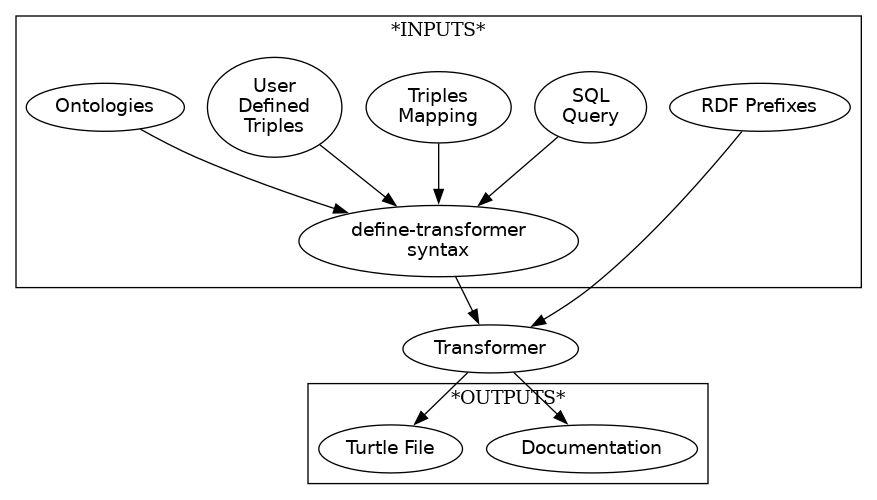
\includegraphics[width=0.7\linewidth]{systemDesign}
  \caption{\textit{Overview of how SQL is converted to RDF and documentation}}
  \label{fig:system-diagram}
  \centering
\end{figure}

Figure \ref{fig:system-diagram} shows the overarching structure of the DSL under consideration.  In general, the transformation from SQL to RDF comprises the processing of distinct input components into a set of outputs: a turtle and markdown file.  These inputs comprise:

\begin{enumerate}
\item \textit{Ontologies}: An ontology is a formal way of representing knowledge.  In the context of Genenetwork, several ontologies are selected to serve as conceptual frameworks for characterizing various entities, including experiments, investigators, species, genes and other relevant entities.
\item \textit{SQL Query}: Acting as the most important instruction set, the SQL query is executed as a pivotal step in the transformation process.
\item \textit{Triples Mapping}: This is a clear mapping between the results of the aforementioned SQL query and the corresponding RDF structure.
\item \textit{User Defined Triples}: In scenarios where existing ontologies fail to encompass domain-specific concepts within the Genenetwork context, user-defined triples are introduced to accommodate these unique conceptual dimensions.
\item \textit{RDF Prefixes}: These are the RDF namespaces that will be appended to the beginning of the turtle file.
\end{enumerate}

\section{Using Scheme to Define the DSL}

GNU Guile, a Scheme dialect, was used to create this DSL since it provides a rich hygienic macro system.  Macros are Scheme's syntactic enhancements which transform an expression in which they are embedded in before evaluation occurs.  From Figure \ref{fig:system-diagram}, the ``define-transformer'' macro is the central driver for converting SQL to RDF.  It provides an interface for specifying the SQL query, user-defined triples, and SQL-to-RDF mapping.  The ``define-transformer'' macro is one of the inputs to the ``transform-with-documentation'' macro which takes objects using the ``define-transformer'' macro as input, along with RDF prefixes.  It then parses the abstract syntax tree of the ``define-transformer'' macro to automatically generate documentation, and executes the transformation itself, resulting in a Turtle file.

Appendix \ref{appendix:sample-program} shows how a a particular program can be defined using the created DSL.  It also shows the example generated markdown documentation and the generated RDF file.

\begin{ack}
This work was supported by African AI Research Awards 2022 
\end{ack}

\bibliographystyle{unsrt}
\bibliography{refs}

\appendix

\section{Appendix}

\subsection{Sample Program that Converts a Table into RDF}
\label{appendix:sample-program}
Here's a small code snippet that demonstrates how one would convert a table called ``Tissue'' with a column ``Tissue.Name'' into RDF:


w
The above snippet generates the following documentation:

\begin{Verbatim}[frame=single]
# Tissue Metadata
## 'tissue'

## Generated Triples:

The following SQL query was executed:

```sql
SELECT Tissue.Short_Name, Tissue.Name FROM Tissue
```

The above query results to triples that have the form:

```text
gn:tissueTissue_short_name -> rdf:type -> gnc:tissue 
gn:tissueTissue_short_name -> rdfs:label -> Tissue(Name) 
```
Here's an example query:

```sparql
PREFIX gn: <http://genenetwork.org/id/> 
PREFIX gnt: <http://genenetwork.org/terms/> 
PREFIX skos: <http://www.w3.org/2004/02/skos/core#> 
PREFIX gnc: <http://genenetwork.org/category/> 
PREFIX rdf: <http://www.w3.org/1999/02/22-rdf-syntax-ns#> 
PREFIX rdfs: <http://www.w3.org/2000/01/rdf-schema#> 

SELECT * WHERE { 
    ?s rdf:type gnc:tissue .
    ?s rdfs:label "Brain mRNA" .
    ?s ?p ?o .
}
```

Expected Result:

```rdf
gn:tissueBrn rdf:type gnc:tissue .
gn:tissueBrn rdfs:label "Brain mRNA" .
```
\end{Verbatim}


The generated turtle (truncated) file is:

\begin{Verbatim}[frame=single]
@prefix gn: <http://genenetwork.org/id/> .
@prefix gnt: <http://genenetwork.org/term/> .
@prefix skos: <http://www.w3.org/2004/02/skos/core#> .
@prefix gnc: <http://genenetwork.org/category/> .
@prefix rdf: <http://www.w3.org/1999/02/22-rdf-syntax-ns#> .
@prefix rdfs: <http://www.w3.org/2000/01/rdf-schema#> .

gnc:tissue a skos:Concept .
gn:tissueBrn rdf:type gnc:tissue .
gn:tissueBrn rdfs:label "Brain mRNA" .
gn:tissueCb rdf:type gnc:tissue .
gn:tissueCb rdfs:label "Cerebellum mRNA" .
[...]
\end{Verbatim}

\end{document}
